\documentclass[11pt]{article}
\usepackage[margin=1in]{geometry}
\usepackage{dirtree}
\usepackage{biblatex}
\bibliography{main} 
\addbibresource{main.bib}
\usepackage{amsmath}
\usepackage{listings}
\usepackage{graphicx}
\usepackage{pythonhighlight}
\usepackage{subfig}
\usepackage{caption}
\usepackage{float}

\author{Francesco Saverio Zuppichini}
\title{Machine Learning - Assignment 1}
\begin{document}
\maketitle

We decided to split the code in the following files in order to decouple the logic and create a better environment booth for developing and testing.
\begin{itemize}
	\item \texttt{skeleton.py} Holds the original function such as \texttt{run\_part1} and \texttt{run\_part2}
	\item \texttt{Perceptron.py} Holds the Perceptron class
	\item \texttt{NeuralNetwork.py} Holds the NeuralNetwork class
	\item \texttt{BetterNeuralNetwork.py} Holds the BetterNeuralNetwork class
	\item \texttt{activation\_function.py} Holds all the activation functions, eg. \texttt{tanh}
	\item \texttt{cost\_functions.py.} Holds all the errors functions, eg. \texttt{MSE}
	\item \texttt{main.py} Main scripts where the functions are called
	\item \texttt{utils.py} A set of utils function 
	\item \texttt{plots.py} Functions used to generate the plots in the report
\end{itemize}

\section{The Perceptron}
\subsection{Question 1}
\subsubsection{Vectorized equations}
Equation \ref{eq:vectorized_perceptron} shows the vectorised equation for a single perceptron

\begin{equation}
\label{eq:vectorized_perceptron}
output = X\times W + b
\end{equation}
Where $X = {x_1, ... x_n}$ is the input set and $W = {w_1, ..., w_n}$ is the target set. We denote $y$ the output of the perceptron.

\subsubsection{Mean Squared Error}
Equation \ref{eq: MSE_perceptron} denotes the Mean Square Error function for our single perceptron
\begin{equation}
\label{eq: MSE_perceptron}
	E(w) = \frac{1}{N}\sum_{i = 1}^N(\underbrace{y(x_i,w_i)}_{\text{predicted}} - \underbrace{t_i}_{\text{actual}})^2)
\end{equation}
One trick that is usual done is to multiply equation $(2)$ by $\frac{1}{2}$, so when we take the derivative the $2$ goes away. This is called One Half Mean Squared Error.

\subsubsection{Derivate of the error with respect to the weights}
In order to reduce our error function we need to compute the first derivative with respect to the weights.\begin{equation}
\frac{\partial E}{\partial w_k}	=\frac{\partial E}{\partial y_i}\frac{\partial y_i}{\partial w_k} =  (w_k \cdot x_{ik} - t) \cdot x_{ik}
\end{equation}
\subsubsection{Compute the new weight values after one step using a learning rate of 0.02}
Since it was not specified that the calculation must be done by hand, we called \texttt{train\_one\_step} in order to compute the new weights, as follows:
\begin{python}
X,T = get_part1_data()
p = Perceptron()
sk.train_one_step(p,0.02,np.array([X[0]]),np.array([T[0]]))
print(p.var['W']) //output weights the values	
print(p.var['b']) //output the new bias value
\end{python}
Where the new weights and bias are
$$W_{k + 1} = \begin{pmatrix}
 0.844 \\
 -0.148
\end{pmatrix}, b_{k+1} = \begin{pmatrix}
	2.044
\end{pmatrix}$$
\subsubsection{Gradient Descend}
The gradient descend is an iterative optimisation algorithm that follows the direction of the negative gradient in order to minimised an objective function. It can be effectively used as Learning Algorithm because it reduces the error function, Equation \ref{eq: MSE_perceptron}, and adjusts the weights properly. Equation \ref{eq: GD} shows the generic update rule.
\begin{equation}
\label{eq: GD}
	w_{k + 1} = w_k - \eta \nabla E(w_k)
\end{equation}
Where $\eta$ is the step size, also called \textbf{learning rate} in Machine Learning. This parameter influences the behaviour of gradient descent, a small number can lead to local minimum, while a bigger learning rate could "over-shoot" and decreasing the converge ration. Later in this project you will see how a wrong $\eta$ can strongly change the output of a Neural Network.

For this reasons, numerous improvements have been proposed to avoid local minima and increase its convergence ration, some of them are: Conjugate Gradient and Momentum.
% TODO if time talk about them
\subsection{Implement the MSE and dMSE}
You can find them in \emph{cost\_functions.py}
\subsection{Implement the function forward and backward}
The \emph{forward} and \emph{backward} function can be found in \emph{Perceptron.py}. You can find \emph{train\_one\_step} in \emph{skeletron.py}.

\subsection{Implement the \emph{run\_part1}}
You can find the implementation in the code, \emph{skeletron.py}. Figure \ref{fig:runPart1} shows the final result after 15 steps using a learning rate of $0.02$. We can notice that the Perceptron worked as aspected since it correctly classified the two colour sets.
\begin{figure}[H]
	\centering
	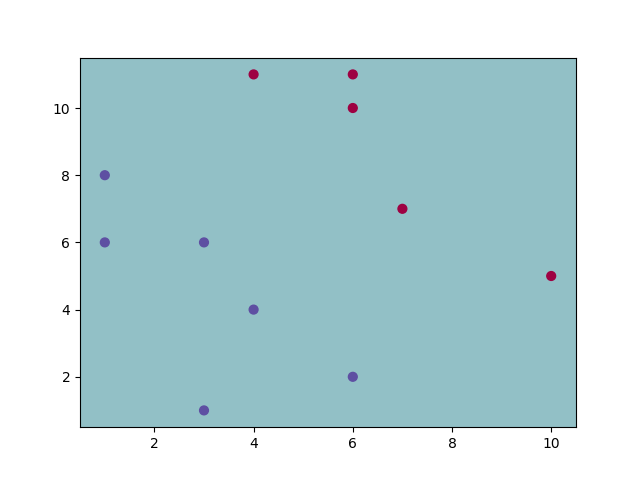
\includegraphics[scale=0.6]{images/run_part1}
	\caption{\emph{run\_part1} plot}
	\label{fig:runPart1}
\end{figure}

\section{A Neural Network}
\subsection{ Implement the activation functions}
You can find them inside \emph{activation\_functions.py}. I have also implemented the \textbf{Relu} that will be used in Section 3.
\subsection{Question 2}
\subsubsection{Forward pass}
In order to calculate the forward pass of a Neural Network we need to compute the activation of each layer, $l$, ad use it as input of the next one until we reach the output layer. 

Equation \ref{eq:forwardPass} shows the activation $a$ of layer $l$ for the $j$-th neuron on that layer.

\begin{equation}
\label{eq:forwardPass}
a^l_j = \sigma(\sum_k w^l_{jk}a^{l-1}_k + b^l_j)
\end{equation}

Where $w^l_{jk}$ is the connection from neuron $k$ in the $l-1$ layer to $j$, $a^{l-1}$ is the activation of the previous layer and $b^l_j$ is the bias of $j$-th neuron in the $l$ layer. With this in mind, we can rewrite \ref{eq:forwardPass} in a efficient vectorised form
\begin{equation}
\label{eq:forwardPassVectorized}
a^l = \sigma(W^la^{l-1} + b^l)
\end{equation}

\subsubsection{Delta rules}
In a Neural Network the weights are iteratively changed in order to decrease the error function, called $E$.Equation \ref{eq:deltaRule_1} defines $\delta^l_j$ as the output error of neuron $j$ in layer $l$
\begin{equation}
	\label{eq: deltaRule_1}
	\delta^l_j = \frac{\partial E}{\partial z^l_j}
\end{equation}
Strictly speaking, $\delta^l_j$, is how much the error function changes by changing the weighted input on that layer. Applying the chain rule, Equation \ref{eq:deltaRule_1} becomes:
\begin{equation}
\label{eq:deltaRule_2}
\delta^l_j = \frac{\partial E}{\partial a^l_j} \frac{\partial a^l_j}{\partial z^l_j}
\end{equation}
By knowing that $a^l_j = \sigma(z^l_j)$, Equation \ref{eq:deltaRule_2} can be expressed as
\begin{equation}
\label{eq:deltaRule}	
\delta^l_j = \frac{\partial E}{\partial a^l_j} \sigma'(z^l_j)
\end{equation}  

 %
%We define $\Delta z^l_j$ the quantity added to the $j$-th neuron's weighted input in the $l$ layer by the network.
% The new output of that neuron becomes $\sigma(z^l_k + \Delta z^l_j)$ causing a changing by $\frac{\delta E}{\delta z^l_k}\Delta z^l_j$. 
\subsubsection{Derivatives of the weights}
We want to compute $\frac{\partial E}{\partial w^l_{jk}}$. Applying the delta rule:
\begin{equation}
\frac{\partial E}{\partial w^l_{jk}} = \frac{\partial E}{\partial z^l_j}\frac{\partial z^l_j}{\partial w^l_{jk}} =	
\frac{\partial E}{\partial a^l_j}\frac{\partial a^l_j}{\partial z^l_{j}}
\frac{\partial z^l_j}{\partial w^l_{jk}}
\end{equation}
\begin{equation}
\label{eq:derivativesWeigthDeltas}	
\frac{\partial E}{\partial w^l_{jk}} = a^{l-1}_k \delta^l_j
\end{equation}
\subsection{Implement the functions forward and backward of the Neural Network class.}
You can find them in \emph{NeuralNetwork.py}
\subsection{Train Network}
\subsubsection{ Split the data into a train set and a test set}
We decided to split the training set and test set with a ratio of 80:20. If we choose a smaller train set we may under-train the network and, on the other hand, if we shrink the test set we may \emph{overfit}. In order to do so, we created a function called \texttt{get\_train\_and\_test\_data} in \emph{utils.py}.

Figure \ref{fig: train_test_set} shows the plot for the train set and the test set. They are created by calling \texttt{twospirals} using competition's configuration.
\begin{figure}[h]
	\centering
	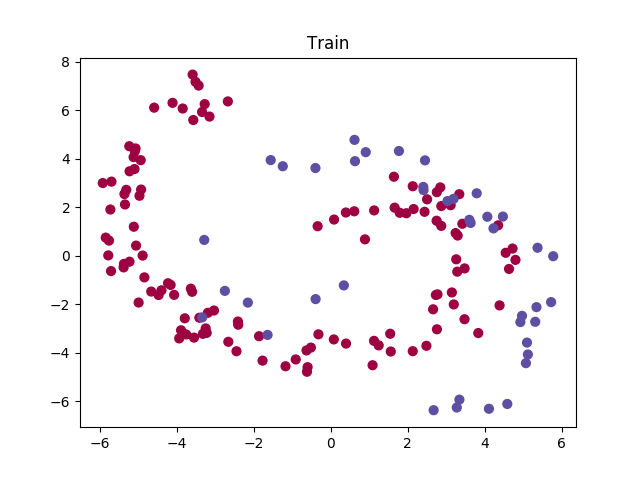
\includegraphics[scale=0.5]{images/train_set}
	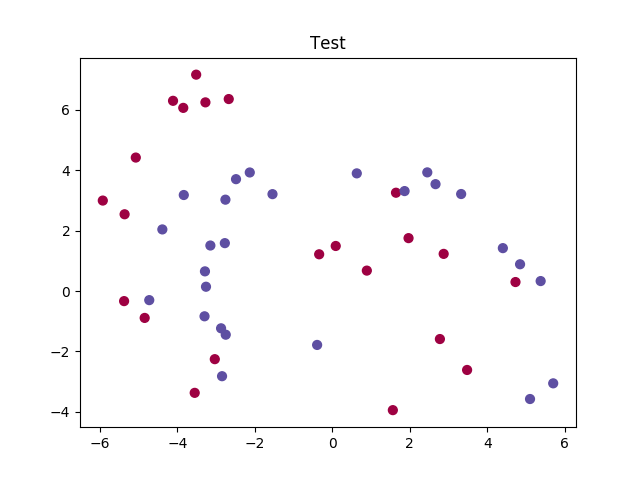
\includegraphics[scale=0.5]{images/test_set}
	\caption{Train set and Test set}
	\label{fig: train_test_set}
\end{figure}


\subsubsection{Initialise the weights randomly and find a good learning rate to train}
In order to find the correct learning rate, we decided to fist test the network with different sizes in order have some empirical data. Figure \ref{fig: learning_rate_convergence} shows the convergence rate with five learning rates. The data was generated using the standard inputs and target from \texttt{twospirals} and then normalised the gradient with its average each 100 iterations in order to provide a smoothed line.

\begin{figure}[H]
\centering
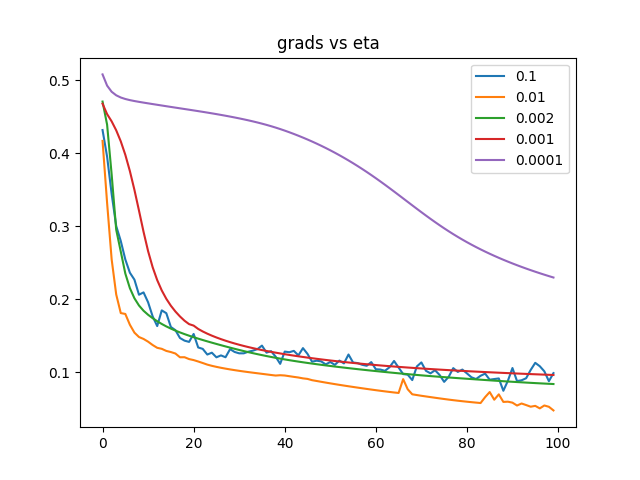
\includegraphics[scale=0.6]{images/NN_boundary_vs_learning_rates/grads}
\caption{Learning rate convergences}
\label{fig: learning_rate_convergence}
\end{figure}

%This little benchmark shows that a big step size, like $0.1$, do not lead to a very stable converge because it overshoots and it cannot find the correct minimum. On the other hand, a very small eta, $0.0001$, converges very slowly and training a model with it will take forever. The best choice is a value between then, $0.01$, $0.002$ or $0.001$.
The benchmark shows that $0.1$ is the best $\eta$ choice since it is the faster and more stable, $0.5$ is also a good choice.
\subsubsection{Plot the learning rate of at least 5 different learning rates on both sets}
Since it was not clear what to plot, we decided to plot five boundaries for the five learning rates used in section 2.4.2. For the benchmark, we used 40.000 iterations that are more than enough to make the model converge to a good solution. Figure \ref{fig: learning_rate_boundary} shows the results
\begin{figure}[H]
	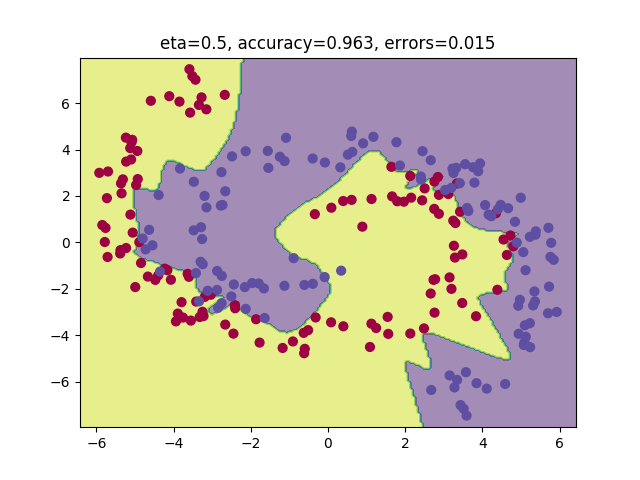
\includegraphics[scale=0.5]{images/NN_boundary_vs_learning_rates/0}
	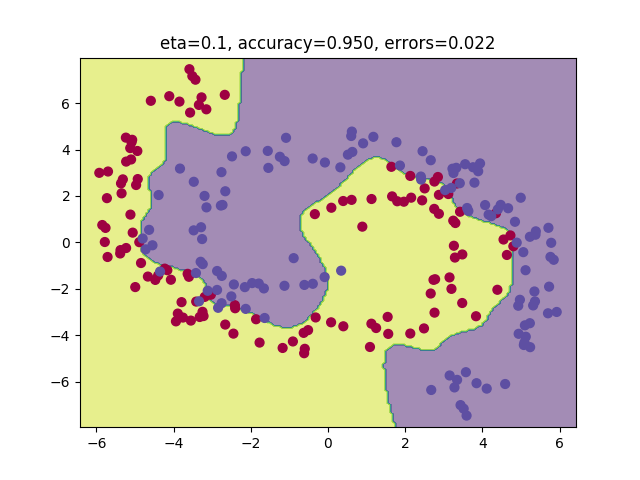
\includegraphics[scale=0.5]{images/NN_boundary_vs_learning_rates/1}
	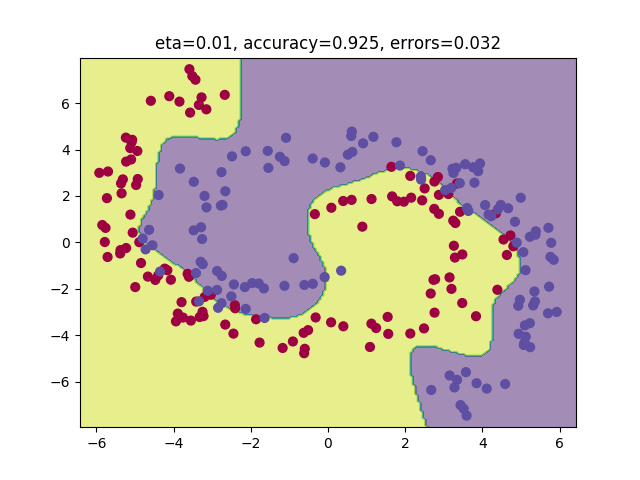
\includegraphics[scale=0.5]{images/NN_boundary_vs_learning_rates/2}
	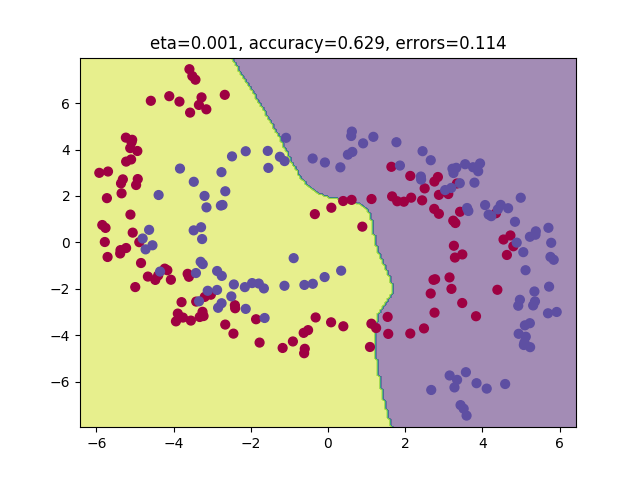
\includegraphics[scale=0.5]{images/NN_boundary_vs_learning_rates/3}
	\centering
	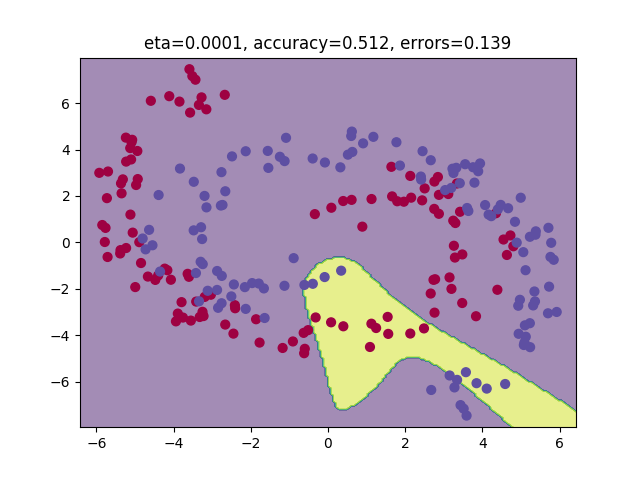
\includegraphics[scale=0.5]{images/NN_boundary_vs_learning_rates/4}
	\caption{model boundary vs learning rates}
	\label{fig: learning_rate_boundary}

\end{figure}
Figure \ref{grad_vs_eta} shows different eta vs gradients and errors respectively

\begin{figure}[H]
\centering
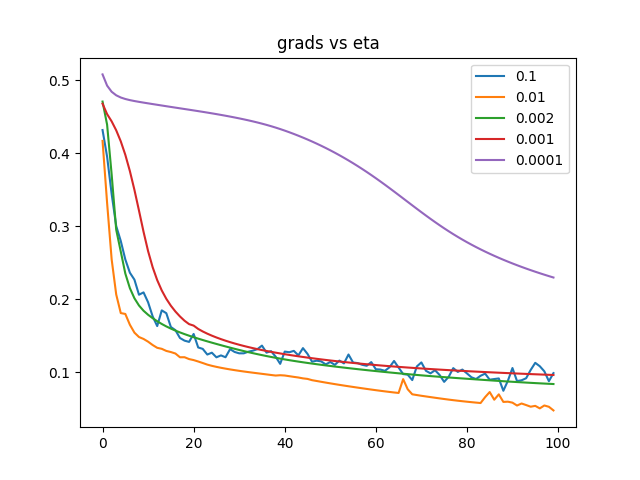
\includegraphics[scale=0.5]{images/NN_boundary_vs_learning_rates/grads}
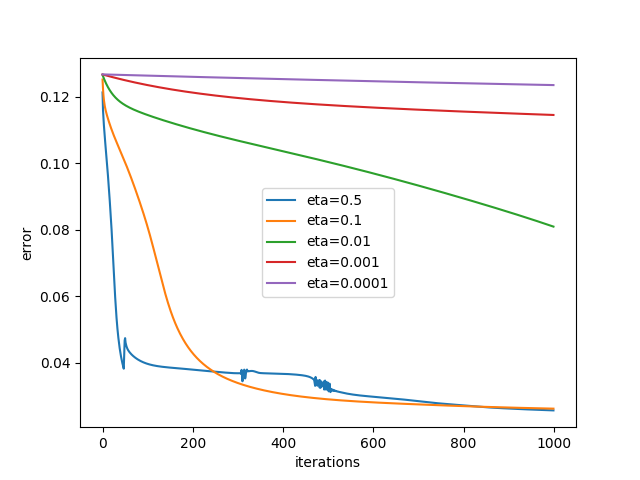
\includegraphics[scale=0.5]{images/NN_boundary_vs_learning_rates/errors}
\caption{eta vs grads and costs}
\label{fig: grad_vs_grads_costs}
\end{figure}

\subsubsection{Plot the boundary of the model which converged the most on the training data}
Figure \ref{fig: NN_MSE_002_boundary} shows the model boundary after reach a MSE error less than $0.02$ using a step size of $0.001$. The network used the following seed: \texttt{1}. You can get the same plot by calling \texttt{run\_part2}.
\begin{figure}[H]
\centering
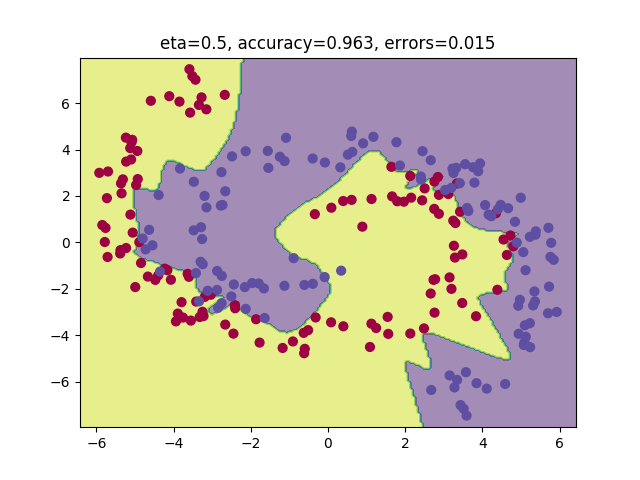
\includegraphics[scale=0.6]{images/NN_boundary_vs_learning_rates/0}	
\caption{Boundary of the model with MSE less than 0.02}
\label{fig: NN_MSE_002_boundary}
\end{figure}
 \subsection{Explain if this is a good model for the data}
The model seems good enough for the data generated by calling \texttt{twospirals} with the standard configuration. however, by using the data for part 3 the model loose lots of accuracy due to its gradient descent implementation that does not prevent the algorithm to fall into local minima. 
A better model is present in detail in the following Section.
\section{Further Improvements}
In this sections we analyse each extension that we tried, even if they did not improve our solution, in order to create a better model.
\subsection{Generic Implementation}
Since the NeuralNetwork class has a fixed number of layers, the first improvement that we did was to create a generic implementation.

The \texttt{BetterNeuralNetwork} class exposes an API allowing the creation of a generic Neural Network by adding and shaping layers.

After instance the class, is it possible to add a input layer by calling \texttt{add\_hnput\_layer(size\_in,size\_out)}. Many hidden layers can be added by using \texttt{add\_hidden\_layer(size\_out)}, the "size\_in" is not necessary since it can be easily calculated by the network. Then method \texttt{add\_output\_layer(size\_out)} adds the output lauer. It follows a full example where we create the same Neural Network from Exercise 2.
\begin{python}
   bnn = BNN()
   bnn.add_input_layer(2, 20, np.tanh, act.dtanh)
   bnn.add_hidden_layer(15, np.tanh, act.dtanh)
   bnn.add_output_layer(1)
\end{python}

For each layer is also possible to specified the activation function, as default value \emph{signmoid} is used. We have also implemented \texttt{relu} and \texttt{dRelu} to try them.

\texttt{BetterNeuralNetwork} exposes \texttt{train} method that performs forward, backpropagation and weight updates directly. It accepts as input the training sets, the targets, max iterations, a dictionary containing the parameters and the gradient descent update method name, the supported ones are: \texttt{'gradient\_descent'} (default), \texttt{'momentum'} and \texttt{'adagrad'}\subsection{Initial weight and bias}
Weight initialisation is crucial to create a good model. I used the following formula.

$$w = random(n)/\sqrt{n}$$

Where $n$ is the size of the input. This ensures that all neurons in the network initially have approximately the same output distribution and empirically improves the rate of convergence. \footnote{http://cs231n.github.io/neural-networks-2/}

Using $numpy$:
\begin{python}
np.random.randn(in_size,out_size)/np.sqrt(in_size)
\end{python}

The bias are initialised with a very small number close to zero, for such reason I scaled down the each random value by a factor of $100$.

\subsection{Performance}
Due to a better and generic implementation, our \texttt{BetterNeuralNetwork} is slightly faster than the one from Section 2. Table \ref{table: performance_NN_BNN} shows the result of a little benchmark
\begin{table}[H]
\centering
  \begin{tabular}{ | l | c | r |}
    \hline
    iterations & time NN & time BNN\\ \hline
    10 & 17.5ms  & 13.7ms \\ \hline
    100 & 134.5ms  & 128.2ms \\ 
    1000 & 461.6ms  & 458.84ms \\ \hline
    10000 & 4455.6ms & 4157.9ms \\ \hline    
  \end{tabular}
  \caption{}
  	\label{table: performance_NN_BNN}

\end{table}
I have also tried to create a small thread pool, so we can save time in thread allocation, in order to parallelise the weight updates, since they are independent operation but without any real advantages. Probably the network is so small that it take more time to call a free thread and submit a work than to compute the operations  sequentially.
\subsection{Momentum}
We used Momentum \cite{Ruder} to speed up the convergence of the network, it prevent getting stuck in local minima and pushes the objective more quickly along the shallow ravine. Basically it give a global direction to the gradient descent based on the previous update. Equation \ref{eq: momentum} shows the new update formula. 

\begin{equation}
	\label{eq: momentum}
	\begin{split}
	\Delta w_{ t + 1} = (\eta \nabla E(w_{t + 1}) + \beta \Delta w_t) \\
	 w_{k + 1} = w_{k + 1} -   \Delta w_{ t + 1}
	 \end{split}
\end{equation}
$\beta \in [0,1]$ is a the momentum factor, usually between $0.5$ and $0.9$. In our benchmarks we used a classic $0.5$. In Figure \ref{fig:momentum}, we can see the converge rate of a classic gradient descent versus momentum for different step sizes. Momentum converges faster in all cases. 
\begin{figure}[H]
\centering
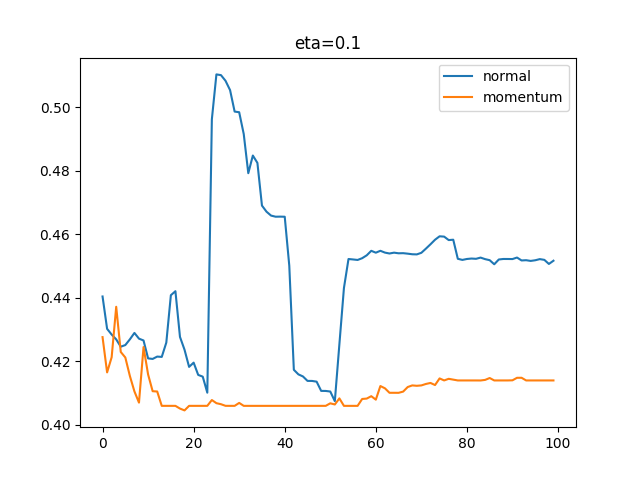
\includegraphics[scale=0.5]{images/momentum/momentum_plot_0.png}	
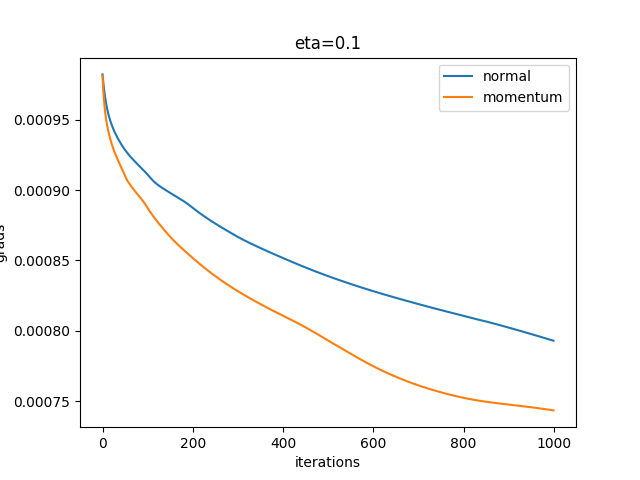
\includegraphics[scale=0.5]{images/momentum/momentum_plot_1.png}	
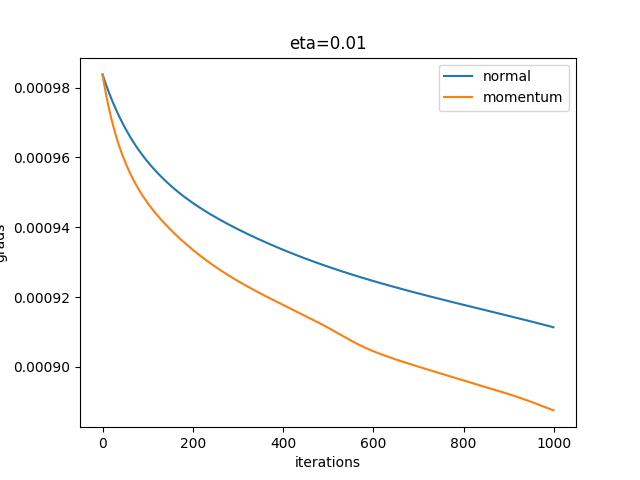
\includegraphics[scale=0.5]{images/momentum/momentum_plot_2.png}	
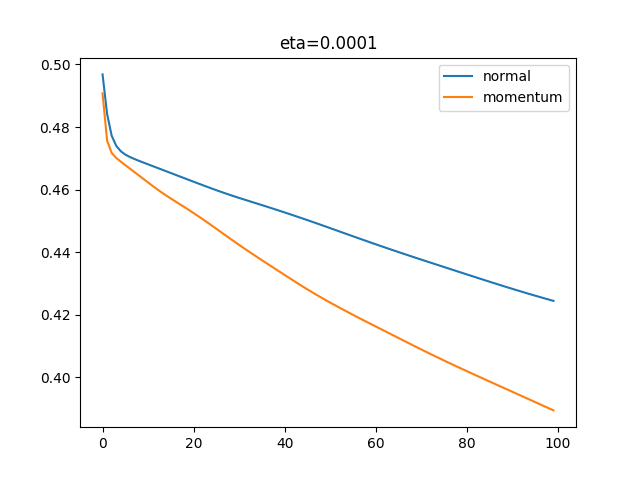
\includegraphics[scale=0.5]{images/momentum/momentum_plot_3.png}	
\caption{Gradient Discent vs Momentum}
\label{fig:momentum}

\end{figure}
In the \texttt{BetterNeuralNetwork} class, momentum can be enabled by passing the correct parameters and type to the \texttt{train} method. The following snippet shows and example

\begin{python}
params = {'eta': 0.01,'beta': 0.5} # beta must be included or the default 0.5 value will be used
nn.train(X_train, T_train, 3000, params, 'momentum')	 # pass 'momentum' as type name
\end{python}

\subsection{Adagrad}
Adagrad \cite{AdaGrad} is an adaptive learning rate algorithm that we implement in order to speed up the convergence. In Figure \ref{fig: adagrad}, we can see the converge rate of a classic gradient descent versus adagrad for different step sizes.
\begin{figure}[H]
\centering
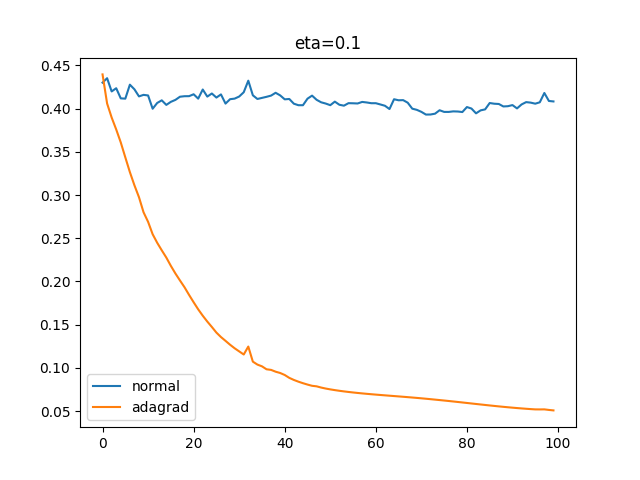
\includegraphics[scale=0.5]{images/adagrad/adagrad_plot_0.png}	
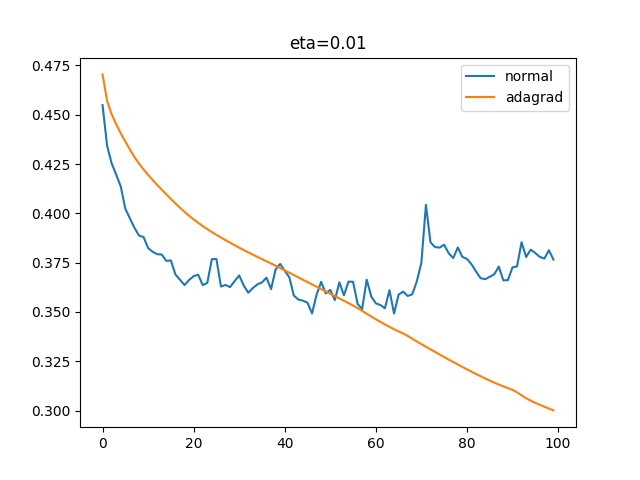
\includegraphics[scale=0.5]{images/adagrad/adagrad_plot_1.png}	
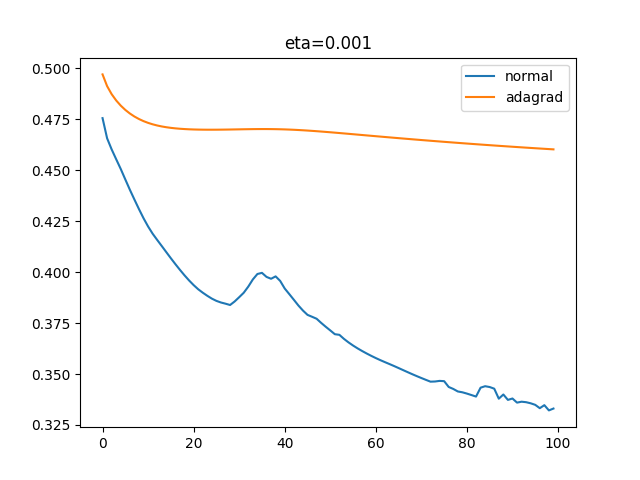
\includegraphics[scale=0.5]{images/adagrad/adagrad_plot_2.png}	
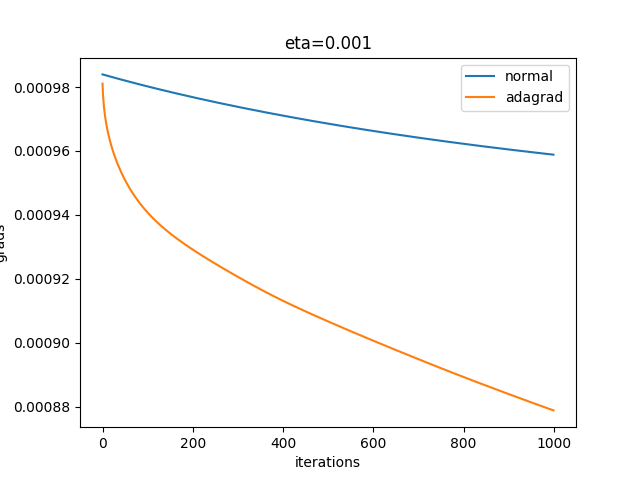
\includegraphics[scale=0.5]{images/adagrad/adagrad_plot_3.png}	
\caption{Gradient Discent vs Adagrad}
\label{fig: adagrad}
\end{figure}
Adagrads works better in any case.
The following snippet shows how to enable it
\begin{python}
nn.train(X_train, T_train, 3000, params, 'adagrad') // pass 'adagrad' as type name
\end{python}

\subsection{Network deep}
Our model is composed by one input layer, three hidden layer and one output layer. We used an empirical approach to find a correct number of hidden layer. We started by make the first layer bigger in order to make our model learn more features about the function. Then we added other three layers, each of them roughly one third smaller than the other. Doing so, our model can recognise more detail about the spiral.

After some tests, we switched to the \textbf{relu} activation function on each layer expect for the output where we used \emph{tanh}. 
%%%%%%%%%%%%%%%%%%% PUT SOME SECTION IN ORDER TO INTRODUCE THE OTHER MERDA CHE HO PROVATO 
We trying other techniques with no luck. We also include them in this report.
\subsection{Stochastic Gradient Descent}
We implemented Stochastic Gradient Descent, it can be enabled by passing the \texttt{batch\_size} value inside the \texttt{params} dictionary

\begin{python}
model.train(train_X, train_T, 4000, { 'eta' : 0.1, 'beta' : 0.5, 'batch_size': 10 }, 'adagrad',testX, testT)	
\end{python}
\subsection{Dropout}
Dropout is a recently introduced regularisation technique. Basically, each node has a probability to be enable on disable in each forward pass. We implemented it by changing the \texttt{forward} method inside \texttt{BetterNeuralNetwork}
\begin{python}
def forward(self, inputs):
    self.A = [inputs]
    self.Z = []
    # dropout probability
    p = 0.5
    
    a = inputs

    for l in self.layers:
        z = a.dot(l.W) + l.b
        # create dropout mask
        u = (np.random.rand(*z.shape) < p) / p
        # apply mask
        z *= u
        a = l.activation(z)
        # store
        self.A.append(a)
        self.Z.append(z)

    return a
\end{python}
At each pass, a binary mask \texttt{u} is created and applied to the layer weighted output \texttt{z}. Unfortunately, this approach did not work well for us and lead to a bad convergence, probably because the network is too small.

\subsection{Results}
Figure \ref{fig: results_boundary} shows the boundary of our new model with one of the best seed: \texttt{0}.
\begin{figure}[H]
\centering
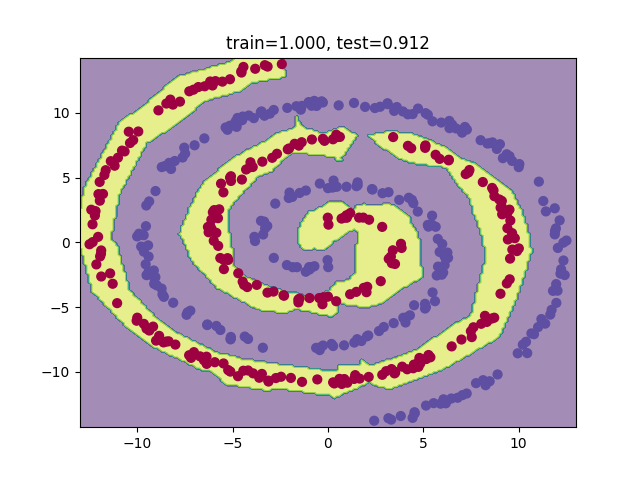
\includegraphics[scale=0.6]{images/competition/competition_0.png}	
\caption{Boundary of the model}
\label{fig: results_boundary}
\end{figure}

The following snippet show our to re-create the model with our API.
\begin{python}
# use same seed
np.random.seed(0)
model = BetterNeuralNetwork()
# create layers
model.add_input_layer(2, 30, act.relu, act.drelu)
model.add_hidden_layer(20, act.relu, act.drelu)
model.add_hidden_layer(15, act.relu, act.drelu)
model.add_hidden_layer(10, act.relu, act.drelu)
model.add_output_layer(1, act.tanh, act.dtanh)

model.train(train_X, train_T , 4000, { 'eta' : 0.1, 'beta' : 0.5 },'adagrad')
\end{python}

%As you may notice we used the \textbf{Adagrad} method.

Figure \ref{fig: bnnVsNn} shows the errors, gradients, error and accuracy for this model with respect to the one from section 2. Obviously the new model is better in every aspect.

\begin{figure}[H]
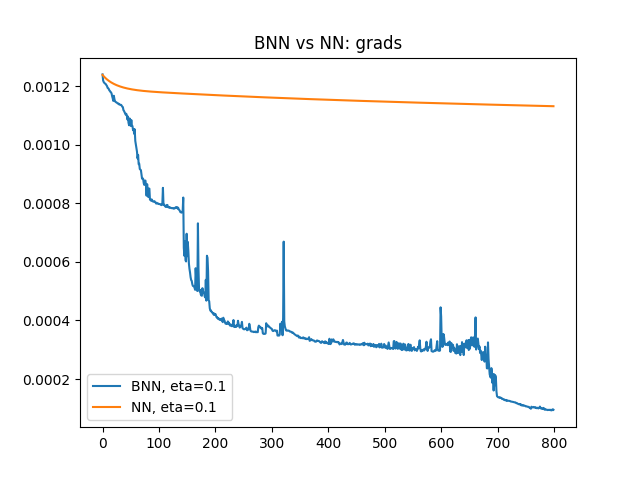
\includegraphics[scale=0.5]{images/BNN_vs_NN/BNN_vs_NN_grads}
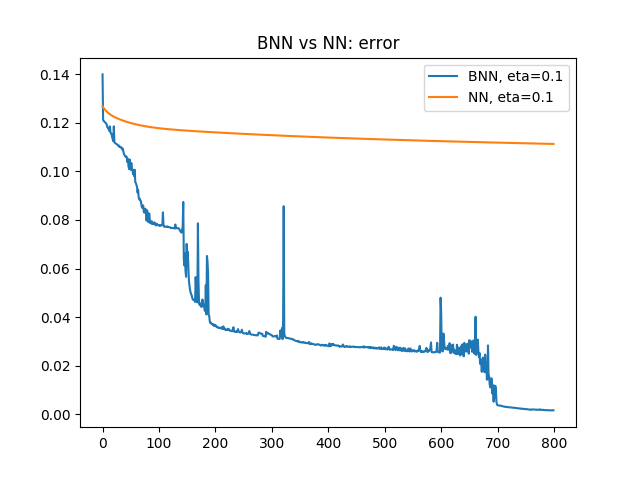
\includegraphics[scale=0.5]{images/BNN_vs_NN/BNN_vs_NN_error}
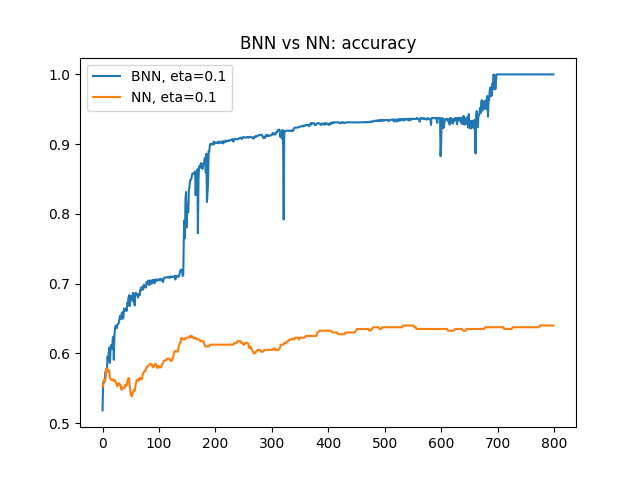
\includegraphics[scale=0.5]{images/BNN_vs_NN/BNN_vs_NN_accuracy}
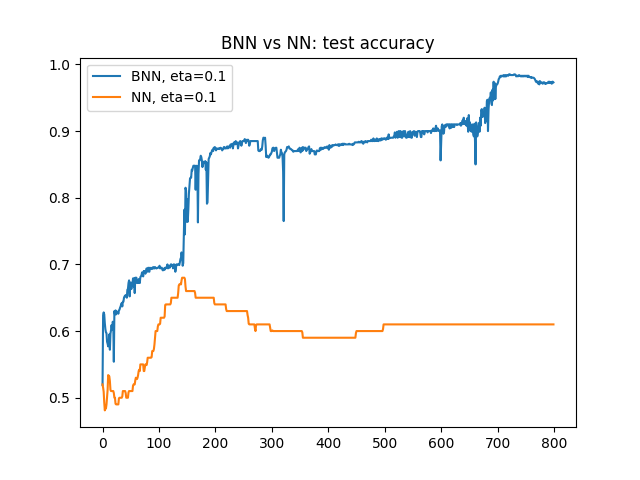
\includegraphics[scale=0.5]{images/BNN_vs_NN/BNN_vs_NN_test_accuracy}
\caption{BetterNeuralNetwork vs Neural Network}
\label{fig: bnnVsNn}

\end{figure}


\begin{figure}[H]
\centering
	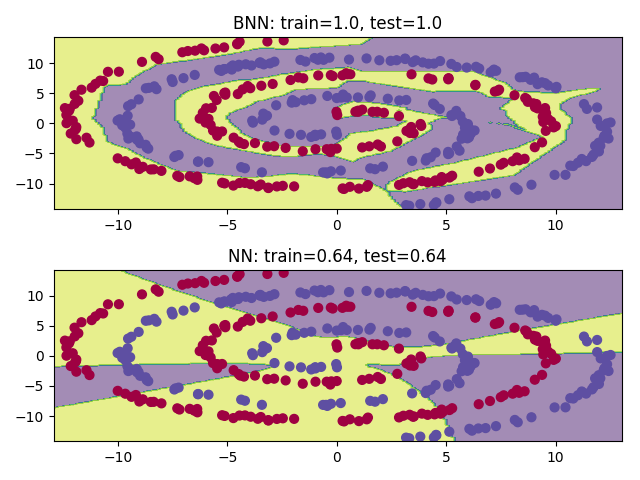
\includegraphics[scale=0.6]{images/BNN_vs_NN/BNN_vs_NN_boundary}
\end{figure}
\subsection{Save and Load}
You can save and load the network state by calling \texttt{.save(file\_name)} \texttt{.load(file\_name}). The following snippet shows hot to load the previous network.

\begin{python}
model = BetterNeuralNetwork()
# create layers
model.add_input_layer(2, 30, act.relu, act.drelu)
model.add_hidden_layer(20, act.relu, act.drelu)
model.add_hidden_layer(15, act.relu, act.drelu)
model.add_hidden_layer(10, act.relu, act.drelu)
model.add_output_layer(1, act.tanh, act.dtanh)
# load prev weights
model.load('competition')
\end{python}

\newpage
\printbibliography

\end{document}
